\documentclass{article}\usepackage[]{graphicx}\usepackage[]{color}
%% maxwidth is the original width if it is less than linewidth
%% otherwise use linewidth (to make sure the graphics do not exceed the margin)
\makeatletter
\def\maxwidth{ %
  \ifdim\Gin@nat@width>\linewidth
    \linewidth
  \else
    \Gin@nat@width
  \fi
}
\makeatother

\definecolor{fgcolor}{rgb}{0.345, 0.345, 0.345}
\newcommand{\hlnum}[1]{\textcolor[rgb]{0.686,0.059,0.569}{#1}}%
\newcommand{\hlstr}[1]{\textcolor[rgb]{0.192,0.494,0.8}{#1}}%
\newcommand{\hlcom}[1]{\textcolor[rgb]{0.678,0.584,0.686}{\textit{#1}}}%
\newcommand{\hlopt}[1]{\textcolor[rgb]{0,0,0}{#1}}%
\newcommand{\hlstd}[1]{\textcolor[rgb]{0.345,0.345,0.345}{#1}}%
\newcommand{\hlkwa}[1]{\textcolor[rgb]{0.161,0.373,0.58}{\textbf{#1}}}%
\newcommand{\hlkwb}[1]{\textcolor[rgb]{0.69,0.353,0.396}{#1}}%
\newcommand{\hlkwc}[1]{\textcolor[rgb]{0.333,0.667,0.333}{#1}}%
\newcommand{\hlkwd}[1]{\textcolor[rgb]{0.737,0.353,0.396}{\textbf{#1}}}%
\let\hlipl\hlkwb

\usepackage{framed}
\makeatletter
\newenvironment{kframe}{%
 \def\at@end@of@kframe{}%
 \ifinner\ifhmode%
  \def\at@end@of@kframe{\end{minipage}}%
  \begin{minipage}{\columnwidth}%
 \fi\fi%
 \def\FrameCommand##1{\hskip\@totalleftmargin \hskip-\fboxsep
 \colorbox{shadecolor}{##1}\hskip-\fboxsep
     % There is no \\@totalrightmargin, so:
     \hskip-\linewidth \hskip-\@totalleftmargin \hskip\columnwidth}%
 \MakeFramed {\advance\hsize-\width
   \@totalleftmargin\z@ \linewidth\hsize
   \@setminipage}}%
 {\par\unskip\endMakeFramed%
 \at@end@of@kframe}
\makeatother

\definecolor{shadecolor}{rgb}{.97, .97, .97}
\definecolor{messagecolor}{rgb}{0, 0, 0}
\definecolor{warningcolor}{rgb}{1, 0, 1}
\definecolor{errorcolor}{rgb}{1, 0, 0}
\newenvironment{knitrout}{}{} % an empty environment to be redefined in TeX

\usepackage{alltt}

\usepackage{amsmath, amssymb}
\usepackage{graphicx}
\usepackage{hyperref}
\usepackage{listings}
\IfFileExists{upquote.sty}{\usepackage{upquote}}{}
\begin{document}

\title{Pol Sci 630:  Problem Set 13 Solutions: Autocorrelation, Clustered SE}
\author{Prepared by: Anh Le (\href{mailto:anh.le@duke.edu}{anh.le@duke.edu})}
\maketitle

\section{Diagnosing autocorrelation}

\subsection{Generating autocorrelated data}

Generate data (i.e. e, X, Y) that follow an AR(2) process, described below. It's an AutoRegressive(2) process because the error term is correlated with itself up to two periods, i.e. $e(t) = a_1e(t-1) + a_2 e(t-2) + v(t)$. (This is also described in slide 4 of your lecture note).

\begin{align}
v(t) &\sim N(0, 1) \\
e(t) &= a_1e(t-1) + a_2 e(t-2) + v(t) \qquad \text{Important: $a_1 + a_2 < 1$} \\
Y(t) &= X(t) + e(t)
\end{align}

Let arbitrarily pick $a_1 = 0.4$, $a_2 = 0.2$, and $T$, the number of time periods, $= 100$

Hint: How do we simulate the vector $e(t)$? Start with $e(1) = rnorm(1), e(2) = a_1 * e(1) + rnorm(1)$, then calculate $e(3), e(4), \dots, e(100)$ according to the DGP above. You may want to use a loop for this.

\textbf{Solution}

\begin{knitrout}
\definecolor{shadecolor}{rgb}{0.969, 0.969, 0.969}\color{fgcolor}\begin{kframe}
\begin{alltt}
\hlstd{T} \hlkwb{<-} \hlnum{100} \hlcom{# Num of time periods}

\hlcom{# Generate autocorrelated e}
\hlstd{e} \hlkwb{<-} \hlkwd{vector}\hlstd{(}\hlkwc{mode} \hlstd{=} \hlstr{'numeric'}\hlstd{,} \hlkwc{length} \hlstd{= T)}
\hlstd{e[}\hlnum{1}\hlstd{]} \hlkwb{<-} \hlkwd{rnorm}\hlstd{(}\hlnum{1}\hlstd{)}
\hlstd{e[}\hlnum{2}\hlstd{]} \hlkwb{<-} \hlnum{0.4} \hlopt{*} \hlstd{e[}\hlnum{1}\hlstd{]} \hlopt{+} \hlkwd{rnorm}\hlstd{(}\hlnum{1}\hlstd{)}
\hlkwa{for} \hlstd{(t} \hlkwa{in} \hlnum{3}\hlopt{:}\hlstd{T) \{}
  \hlstd{e[t]} \hlkwb{<-} \hlnum{0.4} \hlopt{*} \hlstd{e[t} \hlopt{-} \hlnum{1}\hlstd{]} \hlopt{+} \hlnum{0.2} \hlopt{*} \hlstd{e[t} \hlopt{-} \hlnum{2}\hlstd{]} \hlopt{+} \hlkwd{rnorm}\hlstd{(}\hlnum{1}\hlstd{)}
\hlstd{\}}

\hlstd{X} \hlkwb{<-} \hlkwd{rnorm}\hlstd{(T)}
\hlstd{Y} \hlkwb{<-} \hlstd{X} \hlopt{+} \hlstd{e}
\end{alltt}
\end{kframe}
\end{knitrout}

\subsection{Diagnostics: Visual}

Plot residual against time and against lagged , up to 4 lags (e.g. residual ~ lag-1 residual, residual ~ lag-2 residual, etc. up to 4 plots) How does the correlation look across the four plots?

Hint: to create a lagged vector, you can use \verb`lag` in package \verb`dplyr`. In other cases, i.e. generating lags in a data frame / panel, probably best to use \verb`DataCombine` like in the lab tutorial.

\textbf{Solution}

\begin{knitrout}
\definecolor{shadecolor}{rgb}{0.969, 0.969, 0.969}\color{fgcolor}\begin{kframe}
\begin{alltt}
\hlstd{m_auto} \hlkwb{<-} \hlkwd{lm}\hlstd{(Y} \hlopt{~} \hlstd{X)}
\hlstd{e} \hlkwb{<-} \hlkwd{resid}\hlstd{(m_auto)}

\hlkwd{par}\hlstd{(}\hlkwc{mfrow} \hlstd{=} \hlkwd{c}\hlstd{(}\hlnum{2}\hlstd{,} \hlnum{2}\hlstd{))}
\hlkwd{plot}\hlstd{(dplyr}\hlopt{::}\hlkwd{lag}\hlstd{(e,} \hlnum{1}\hlstd{), e)}
\hlkwd{plot}\hlstd{(dplyr}\hlopt{::}\hlkwd{lag}\hlstd{(e,} \hlnum{2}\hlstd{), e)}
\hlkwd{plot}\hlstd{(dplyr}\hlopt{::}\hlkwd{lag}\hlstd{(e,} \hlnum{3}\hlstd{), e)}
\hlkwd{plot}\hlstd{(dplyr}\hlopt{::}\hlkwd{lag}\hlstd{(e,} \hlnum{4}\hlstd{), e)}
\end{alltt}
\end{kframe}
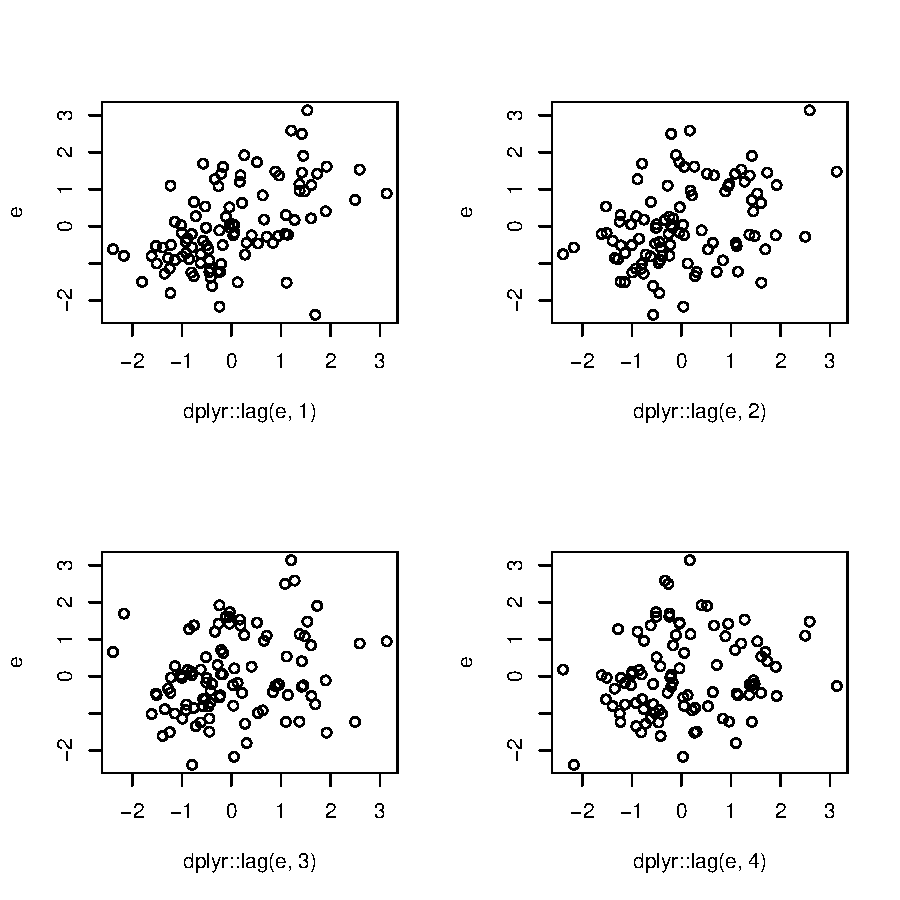
\includegraphics[width=\maxwidth]{figure/unnamed-chunk-2-1} 

\end{knitrout}

We see that he error autocorrelation diminishes the further the lag is (See how the relationship is very strong in the first plot, but not so much in the fourth?).

\subsection{Diagnostics: Hypothesis testing}

Regress residuals against X and lag1 and lag2 residuals, and then doing an F test for joint significance in the lagged residuals. (This is described in slide 4 of your lecture note).

You can use \verb`linearHypothesis` function in package \verb`car` to conduct a joint F test.

\textbf{Solution}

\begin{knitrout}
\definecolor{shadecolor}{rgb}{0.969, 0.969, 0.969}\color{fgcolor}\begin{kframe}
\begin{alltt}
\hlstd{lag1_e} \hlkwb{<-} \hlstd{dplyr}\hlopt{::}\hlkwd{lag}\hlstd{(e,} \hlnum{1}\hlstd{)}
\hlstd{lag2_e} \hlkwb{<-} \hlstd{dplyr}\hlopt{::}\hlkwd{lag}\hlstd{(e,} \hlnum{2}\hlstd{)}

\hlcom{# Reg residual against X and lagged residuals}
\hlstd{m_autotest} \hlkwb{<-} \hlkwd{lm}\hlstd{(e} \hlopt{~} \hlstd{X} \hlopt{+} \hlstd{lag1_e} \hlopt{+} \hlstd{lag2_e)}

\hlcom{# Doing an F test}
\hlkwd{library}\hlstd{(car)} \hlcom{# to run F-test}
\hlkwd{linearHypothesis}\hlstd{(m_autotest,} \hlkwd{c}\hlstd{(}\hlstr{"lag1_e"}\hlstd{,} \hlstr{"lag2_e"}\hlstd{))}
\end{alltt}
\begin{verbatim}
## Linear hypothesis test
## 
## Hypothesis:
## lag1_e = 0
## lag2_e = 0
## 
## Model 1: restricted model
## Model 2: e ~ X + lag1_e + lag2_e
## 
##   Res.Df     RSS Df Sum of Sq      F    Pr(>F)    
## 1     96 118.292                                  
## 2     94  85.157  2    33.135 18.288 1.957e-07 ***
## ---
## Signif. codes:  0 '***' 0.001 '**' 0.01 '*' 0.05 '.' 0.1 ' ' 1
\end{verbatim}
\end{kframe}
\end{knitrout}

We reject the null of no autocorrelation. Notice how we can do the F-test on more than just one lag to detect autocorrelation. In real research, you would use your judgement to guess the autocorrelation structure (i.e. how far back does the autocorrelation go?) and test it.


\section{Clustered errors}

\subsection{Conceptual: Why is it a problem?}

Note: Just me explaining here, nothing for you to do.

Among the \href{https://en.wikipedia.org/wiki/Ordinary_least_squares#Assumptions}{5 assumptions of classical linear regression}, which one was violated by clustered standard errors?

Clustered errors violate the Spherical Error assumption, specifically the No Autocorrelation part, i.e. $E[\epsilon_i\epsilon_j|X] = 0 for i \neq j$. Indeed, clustered errors mean that two observations within the same clusters have correlated error. In other words, $E[\epsilon_i\epsilon_j|X] \neq 0$ if $i, j$ are in the same cluster.

This violation leads to higher standard errors, i.e. higher uncertainty in our model estimates. Intuitively, if clustered errors are present, units within a cluster are correlated. Thus, each unit does not present a 100\% new piece of information. In this case, we have less information to estimate our model, and we are less certain about our estimate.

For example, our cluster is a classroom, and our unit is a student. Imagine the extreme case when every student is a clone of one person. The correlation between units within a classroom is 1 (its maximum). Even if we may have 100-student classroom, there is in fact only one person, one piece of information.

\subsection{Clustered errors and diff-in-diff design}

Describe a diff-in-diff design (briefly, an equation + a few sentences should be enough). Explain why clustered errors is a problem for diff-in-diff.

\textbf{Solution}

A diff-in-diff design:

$$
y_{i, t} = \beta_0 + \beta_1 time_t + \beta_2 treat_i + \beta_3 time_t \times treat_i + \epsilon_{i, t}
$$

where $i$ denotes the unit, and $t$ denotes the time. We have clustered errors here because $\epsilon_{i, t}$ are very likely to be correlated within the same unit $i$. This can happen if I fail to control for an important covariate, thus systematically under- or over-estimate the outcome in a unit $i$.

\subsection{Dealing with clustered errors}

Given the discussion above, it's now common practice to use clustered standard errors with a diff-in-diff design. Indeed, Eddy does in his own work, "The Impact of Recentralization on Public Services: A Difference-in-Differences Analysis of the Abolition of Elected Councils in Vietnam." We'll replicate the first 2 columns in table 2, his main findings.

\textbf{Put results in a stargazer table, including BOTH non-clustered and clustered SE. The final table should 4 columns. How do clustered errors change the size of the coefficient and the SEs?}

How to do it? You have two choices:

1. ``We do these things not because they are easy but because they are hard.'' \href{https://dataverse.harvard.edu/dataset.xhtml?persistentId=doi:10.7910/DVN/IUG2C4}{Here} is the link to Eddy's replication data and code. Figure out yourself how to replicate.

Easier choice after the break. Resist the easier choice.

\pagebreak

2. You can follow these steps. The main findings code is in \verb`APSR_30indicators_0810.do`

\begin{itemize}
\item Load data \verb`panel_commune_2008_2010.dta`
\item Drop Vietnam's Central Highland (\verb`reg8 == 6`) from dataset
\item Create a city dummy, which equals 1 if \verb`tinh==1 | tinh==31 | tinh==48 | tinh==92 | tinh==79`
\item Run regression. Dependent vars: goodroadv, transport. Ind vars: time + treatment + time:treatment + lnarea + lnpopden + city + regional fixed effects. (reg8 is the region ID).
\item Calculate clustered standard errors with multivcov and coeftest. Note that Eddy clustered both by tinh and huyen at the same time. (Tinh and Huyen are province and district in VNese).
\end{itemize}

\textbf{Solution}

\begin{knitrout}
\definecolor{shadecolor}{rgb}{0.969, 0.969, 0.969}\color{fgcolor}\begin{kframe}
\begin{alltt}
\hlkwd{library}\hlstd{(haven) ;} \hlkwd{library}\hlstd{(dplyr) ;} \hlkwd{library}\hlstd{(multiwayvcov) ;} \hlkwd{library}\hlstd{(lmtest)}
\hlstd{d} \hlkwb{<-} \hlkwd{read_dta}\hlstd{(}\hlstr{"panel_commune_2008_2010.dta"}\hlstd{)}

\hlcom{#* Drop Central Highland drop if reg8==6}
\hlstd{d} \hlkwb{<-} \hlstd{d} \hlopt \hlkwd{filter}\hlstd{(reg8} \hlopt{!=} \hlnum{6}\hlstd{)}

\hlcom{# gen city=(tinh==1 | tinh==31 | tinh==48 | tinh==92 | tinh==79)}
\hlstd{d}\hlopt{$}\hlstd{city} \hlkwb{<-} \hlstd{d}\hlopt{$}\hlstd{tinh} \hlopt{==} \hlnum{1} \hlopt{|} \hlstd{d}\hlopt{$}\hlstd{tinh} \hlopt{==} \hlnum{31} \hlopt{|} \hlstd{d}\hlopt{$}\hlstd{tinh}\hlopt{==}\hlnum{48} \hlopt{|} \hlstd{d}\hlopt{$}\hlstd{tinh}\hlopt{==}\hlnum{92} \hlopt{|} \hlstd{d}\hlopt{$}\hlstd{tinh}\hlopt{==}\hlnum{79}

\hlcom{# global inde time treatment time_treatment lnarea lnpopden city i.reg8}
\hlcom{# xi: ivreg2 goodroadv $inde, cluster(tinh huyen)}
\hlstd{m_road} \hlkwb{<-} \hlkwd{lm}\hlstd{(goodroadv} \hlopt{~} \hlstd{time} \hlopt{+} \hlstd{treatment} \hlopt{+} \hlstd{time}\hlopt{:}\hlstd{treatment} \hlopt{+} \hlstd{lnarea} \hlopt{+}
               \hlstd{lnpopden} \hlopt{+} \hlstd{city} \hlopt{+} \hlkwd{factor}\hlstd{(reg8),} \hlkwc{data} \hlstd{= d)}
\hlstd{vcov_road} \hlkwb{<-} \hlkwd{cluster.vcov}\hlstd{(m_road,} \hlkwc{cluster} \hlstd{= d[,} \hlkwd{c}\hlstd{(}\hlstr{"tinh"}\hlstd{,} \hlstr{"huyen"}\hlstd{)])}

\hlstd{m_transport} \hlkwb{<-} \hlkwd{lm}\hlstd{(transport} \hlopt{~} \hlstd{time} \hlopt{+} \hlstd{treatment} \hlopt{+} \hlstd{time}\hlopt{:}\hlstd{treatment} \hlopt{+} \hlstd{lnarea} \hlopt{+}
               \hlstd{lnpopden} \hlopt{+} \hlstd{city} \hlopt{+} \hlkwd{factor}\hlstd{(reg8),} \hlkwc{data} \hlstd{= d)}
\hlstd{vcov_transport} \hlkwb{<-} \hlkwd{cluster.vcov}\hlstd{(m_transport,} \hlkwc{cluster} \hlstd{= d[,} \hlkwd{c}\hlstd{(}\hlstr{"tinh"}\hlstd{,} \hlstr{"huyen"}\hlstd{)])}
\end{alltt}
\end{kframe}
\end{knitrout}

\begin{kframe}
\begin{alltt}
\hlkwd{library}\hlstd{(stargazer)}
\end{alltt}


{\ttfamily\noindent\itshape\color{messagecolor}{\#\# \\\#\# Please cite as:}}

{\ttfamily\noindent\itshape\color{messagecolor}{\#\#\ \ Hlavac, Marek (2015). stargazer: Well-Formatted Regression and Summary Statistics Tables.}}

{\ttfamily\noindent\itshape\color{messagecolor}{\#\#\ \ R package version 5.2. http://CRAN.R-project.org/package=stargazer}}\begin{alltt}
\hlkwd{stargazer}\hlstd{(m_road,} \hlkwd{coeftest}\hlstd{(m_road, vcov_road),}
          \hlstd{m_transport,} \hlkwd{coeftest}\hlstd{(m_transport, vcov_transport),}
          \hlkwc{omit} \hlstd{=} \hlstr{"factor"}\hlstd{,}
          \hlkwc{order} \hlstd{=} \hlkwd{c}\hlstd{(}\hlstr{"time$"}\hlstd{,} \hlstr{"treatment$"}\hlstd{,} \hlstr{"time:treatment"}\hlstd{))}
\end{alltt}
\end{kframe}
% Table created by stargazer v.5.2 by Marek Hlavac, Harvard University. E-mail: hlavac at fas.harvard.edu
% Date and time: Fri, Dec 02, 2016 - 09:36:22 AM
\begin{table}[!htbp] \centering 
  \caption{} 
  \label{} 
\begin{tabular}{@{\extracolsep{5pt}}lcccc} 
\\[-1.8ex]\hline 
\hline \\[-1.8ex] 
 & \multicolumn{4}{c}{\textit{Dependent variable:}} \\ 
\cline{2-5} 
\\[-1.8ex] & goodroadv &   & transport &   \\ 
\\[-1.8ex] & \textit{OLS} & \textit{coefficient} & \textit{OLS} & \textit{coefficient} \\ 
 & \textit{} & \textit{test} & \textit{} & \textit{test} \\ 
\\[-1.8ex] & (1) & (2) & (3) & (4)\\ 
\hline \\[-1.8ex] 
 time & $-$0.007 & $-$0.007 & $-$0.065$^{***}$ & $-$0.065$^{***}$ \\ 
  & (0.012) & (0.013) & (0.014) & (0.018) \\ 
  & & & & \\ 
 treatment & $-$0.104$^{***}$ & $-$0.104$^{**}$ & $-$0.089$^{***}$ & $-$0.089$^{*}$ \\ 
  & (0.025) & (0.051) & (0.028) & (0.052) \\ 
  & & & & \\ 
 time:treatment & 0.086$^{**}$ & 0.086$^{**}$ & 0.102$^{***}$ & 0.102$^{*}$ \\ 
  & (0.035) & (0.037) & (0.038) & (0.053) \\ 
  & & & & \\ 
 lnarea & 0.015 & 0.015 & 0.102$^{***}$ & 0.102$^{***}$ \\ 
  & (0.014) & (0.023) & (0.016) & (0.018) \\ 
  & & & & \\ 
 lnpopden & 0.098$^{***}$ & 0.098$^{***}$ & 0.116$^{***}$ & 0.116$^{***}$ \\ 
  & (0.012) & (0.016) & (0.013) & (0.022) \\ 
  & & & & \\ 
 city & $-$0.031 & $-$0.031 & 0.020 & 0.020 \\ 
  & (0.024) & (0.032) & (0.027) & (0.040) \\ 
  & & & & \\ 
 Constant & 0.352$^{***}$ & 0.352$^{***}$ & $-$0.068 & $-$0.068 \\ 
  & (0.094) & (0.126) & (0.104) & (0.156) \\ 
  & & & & \\ 
\hline \\[-1.8ex] 
Observations & 4,126 &  & 4,126 &  \\ 
R$^{2}$ & 0.140 &  & 0.146 &  \\ 
Adjusted R$^{2}$ & 0.138 &  & 0.144 &  \\ 
Residual Std. Error (df = 4113) & 0.370 &  & 0.410 &  \\ 
F Statistic (df = 12; 4113) & 56.022$^{***}$ &  & 58.819$^{***}$ &  \\ 
\hline 
\hline \\[-1.8ex] 
\textit{Note:}  & \multicolumn{4}{r}{$^{*}$p$<$0.1; $^{**}$p$<$0.05; $^{***}$p$<$0.01} \\ 
\end{tabular} 
\end{table} 


Clustered SEs do not change coefficient size, but inflate the SE. Also, Eddy is an upstanding scholar whose results replicate.

\end{document}
